\chapter{Обзор системы VLC}

\section{Li-Fi и VLC}

\Abbrev{IM}{intensity modulation}
\Abbrev{DD}{direct detection}
\Abbrev{IEEE (Institute of Electrical and Electronics Engineers)}{институт электроники и инжинеров электроники}

Концепт VLC был представлен Гаральдом Хаасом на конференции TED Talk в 2011 году~\cite{Haas2011}. Было предложено использование модуляции интенсивности излучения \--- IM (intensity modulation), а для приёмника (фотодетектор) применять прямое детектирование \--- DD (direct detection). Работа такой системы описывается стандартом IEEE 802.15.7~\cite{IEEE2018}. VLC предлагается использовать как замену проводам и волокну для передачи данных~\cite{Haas16}, а именно для соединения формата <<от точки к точке>>, то есть предполагается, что каждый передатчик соединен только с одним приёмником.

Этот формат соединения и отличается VLC от Li-Fi: последний описывает сеть с двусторонней коммуникацией и наличием многих передатчиком и приёмников, предполагается соединение между одним источником и многими приёмниками \--- соединение формата <<от многих точек к точке>>. Такой тип соединения схож с уже существующим и широко распространенным протоколом Wi-Fi: он тоже позволяет обеспечить мобильность пользователей и незаметное переключение между передатчиками. По сути, стандарт Li-Fi включает в себя стандарт VLC, то проиллюстрировано на схеме~\ref{fig:vlcvslifi}.

\begin{figure}[!ht]
    \centering
    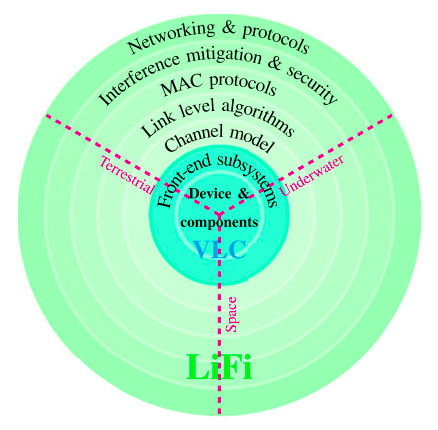
\includegraphics[width=.6\textwidth]{inc/img/vlcvslifi.png}
    \caption{Принципиальная схема Li-Fi и VLC~\cite{Haas16}}
    \label{fig:vlcvslifi}
\end{figure}

\section{Li-Fi передатчик}



Зачастую в системах передачи информации с помощью видимого света в качестве передатчика выбирается светодиодный светильник\footnote{LED luminaire}~\cite{LeMinh2008,Komine2006,Komine2004}. Он представляет из себя полноценное осветительное устройство, состоящее из LED источник излучения, балласта, корпуса и других компонентов. LED источник может состоять из одного или нескольких светодиодов, которые управляются с помощью управляющей микросхемы \--- контроллера, который контролирует ток, питающий светодиод и меняющий его яркость. Когда светодиодный светильник используется для коммуникации, контроллер модернизируется для передачи данных с помощью модуляции излучения. Примером простейшей модуляции является On-Off Keying, то есть <<нули>> и <<единицы>> передаются как два разных уровня интенсивности света.

Важнейшим преимуществом Li-Fi системы является возможность использования её для освещения вместо обычных светильников. В таком случае, функции передачи информации и освещения не должны мешать работе друг друга. Белый свет является превалирующим, так как при таком освещении цвет предметов выглядит естественным, как при солнечном освещении. Для освещений внутри и снаружи помещений всё чаще применяют LED светодиоды, так как они являются экономичными и надёжными. Тогда белый свет можно получить следующими способами:

\Abbrev{LD (laser diode)}{лазерный диод}

\begin{enumerate}
    \item Синий светодиод с фосфором \--- это источник света, состоящий из синего InGaN светодиода, покрытого жёлтым фосфором. Синий свет от источника поглощается фосфором и переизлучается на широком спектре от красного до зелёного, тем самым генерируя белый свет. Изменение цветовой температуры излучаемого света достигается за счёт изменения толщины фосфорного покрытия. 
    \item RGB светодиод \--- это три светодиода (красный, синий и зелёный), при смешении света от которых, получается белый свет. Этот тип светодиодов подходит для Li-Fi систем, чем фосфорные светодиоды, так как последние значительно ограничены временем релаксации фосфора, что может снизить скорость передачи данных (так как оказывается невозможно модулировать интенсивность такого светодиода с частотой выше нескольких МГц~\cite{Khalid2012}). Кроме того, при использовании RGB светодиодов возможно применение цветовой манипуляции \--- метода модуляции с разделением каналов по длинам волн, что позволяет повысить скорость передачи данных~\cite{Bian2019} (раздел \ref{CSK}).
    \item Лазерный диод (LD) \--- в 2011 году в лаборатории Sandia~\cite{Neumann2011} предложили использовать комбинацию четырёх цветных лазерных диодов (красный, синий, зелёный, жёлтый) для получения белого света. Авторы получили очень яркий собранный пучок света, который хорошо подходит для освещения мест, требующих высокую освещенность. Так как лазерное излучение может нанести вред человеку (и из-за коллимированности плохо освещает большую площадь), авторы использовали рассеиватели. Полученное излучение уже не имеет некоторых лазерных характеристик, однако лазерные диоды являются значительно более эффективными, чем RGB светодиоды. В~\cite{Hussein2015} авторы использовали три лазерных диода (рисунок~\ref{fig:ld}) для создания источника света для VLC системы. Они смогли добиться скорости передачи данных до 5 Гб/с. 
\end{enumerate}

\begin{figure}[!ht]
    \centering
    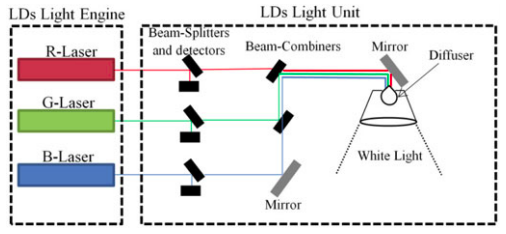
\includegraphics[width=.7\textwidth]{inc/img/ld.png}
    \caption{Принципиальная схема источника в VLC системе в~\cite{Hussein2015} с использованием лазерных диодов. В левой части схемы изображены три цветных лазера: красный, синий и зелёный соответственно; в правой части: разделители пучка и детекторы, устройства для совмещения лучей, зеркало, рассеиватель. На выходе получается свет белого цвета.}
    \label{fig:ld}
\end{figure}

\section{Li-Fi приёмник}

В качестве приёмников в Li-Fi системах чаще всего используются

\begin{enumerate}
    \item фотодетекторы \--- фотодиоды,
    \item датчики изображения \--- камеры.
\end{enumerate}

Фотодетектор \--- полупроводниковое устройство, которое генерирует ток при падении на него света. Современные коммерческие фотодетекторы могут детектировать с частотой до десятков МГц. 

\Abbrev{FPS (frames per second)}{кадры в секунду}

Кроме фотодетекторов, возможно применение камер, которые уже есть в большинстве техники (смартфоны, планшеты, ноутбуки), что может упростить интеграцию этих устройств в Li-Fi систему. Кроме того, возможно применение Li-Fi для передачи информации в рамках интернета вещей~\cite{Duquel2018}. Возможность использовать потребительские камеры появляется из-за того, что камера представляет из себя матрицу фотодиодов. Важным отличием является их количество, что делает быстрый сбор и обработку информации с них затруднительным. Это связано со снимаемой камерой частотой кадров в секунду. Несмотря на значительные ограничения по пропускной способности, есть способы повышения скорости приёма информации, например \--- использование эффекта Rolling shutter~\cite{TRAN2018}. Этот эффект заключается в следующем: так как количество пикселей в камере велико, считывание информации с них происходит построчно (или по столбцам). Если модулировать излучение с периодом, меньшим, чем время считывания одного столбца (строки), то в каждом столбце (строке) будет информация о передаче символа.

Тем не менее, использование фотодиодов остается более предпочтительным, так как с использованием их возможно достижение скорости передачи данных в несколько Гб/с~\cite{Cossu2012}.


